\section{Methods}
\label{sec:methods}

Following the framing of Section~\ref{sec:related-work}, the method proceeds
in five steps, summarized in Figure~\ref{fig:pipeline-overview} and
Table~\ref{tab:rq-method-map}. First, official telemetry is reconstructed
into a phase-aligned STDB (Subsection~\ref{sec:methods-data}). Second, each
team and phase is summarized into one feature row covering trajectory, zone
exposure, combat, and readiness (Subsection~\ref{sec:methods-features}).
Third, inter-team relations are encoded as dynamic team graphs
(Subsection~\ref{sec:team-graphs}); these three steps answer RQ1. Fourth, a leakage-safe next-phase hazard task is
defined on the feature rows (Subsection~\ref{sec:prediction-task}). Fifth,
DynamicSTGNN tests whether the graph relations add predictive signal
(Subsection~\ref{sec:dynamic-team-graph-model}); these two steps answer RQ2.

\begin{figure*}[t]
\centering
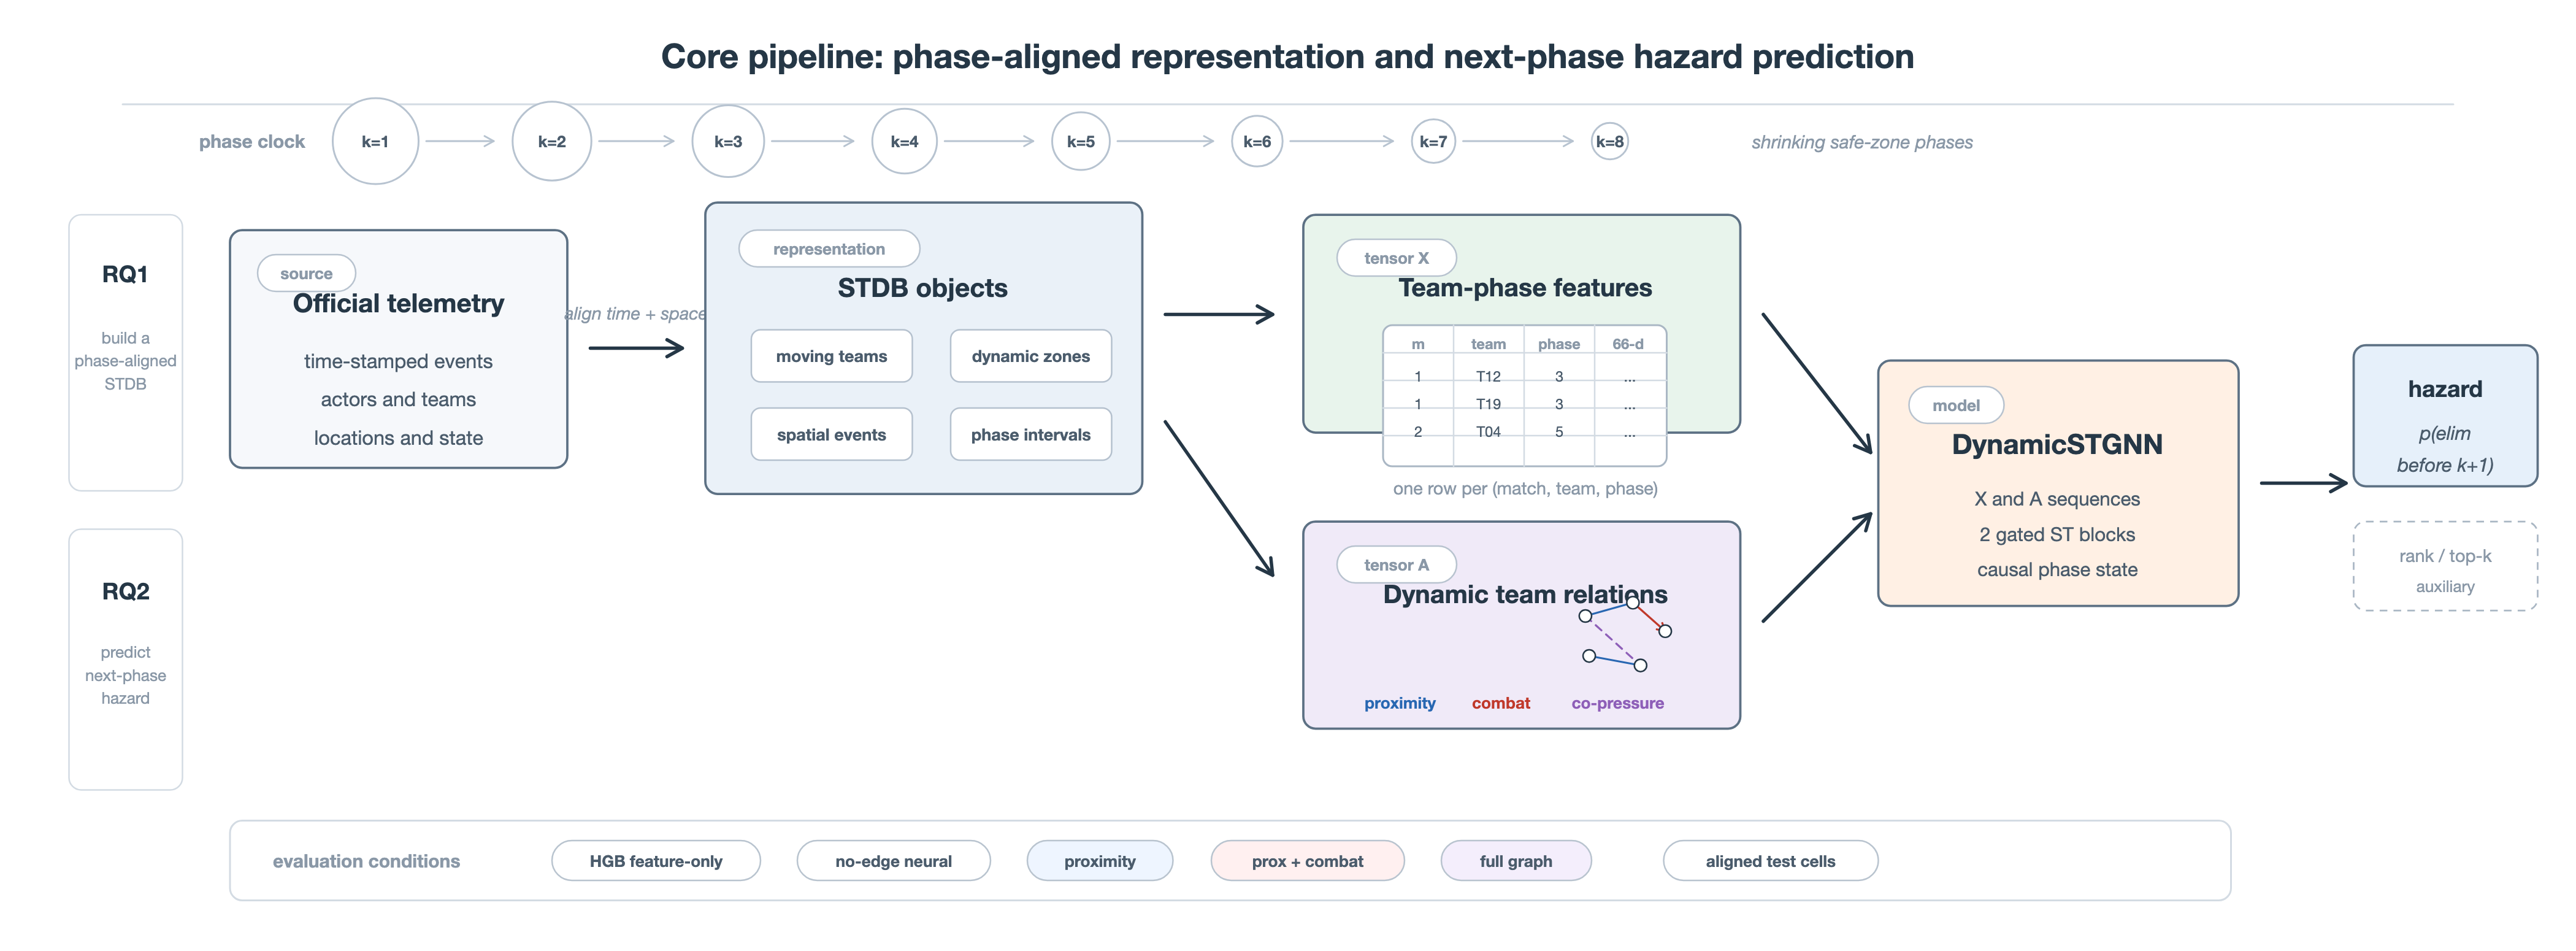
\includegraphics[width=0.86\textwidth]{figures/pipeline_overview.png}
\caption{Pipeline overview. Official telemetry is reconstructed into a
phase-aligned STDB and summarized into team-phase features and dynamic team
graphs (RQ1); DynamicSTGNN is then evaluated against feature-only models for
next-phase elimination hazard (RQ2).}
\label{fig:pipeline-overview}
\end{figure*}

\begin{table}[t]
\centering
\caption{Method pipeline.}
\label{tab:rq-method-map}
\small
\begin{tabular}{p{0.12\linewidth}p{0.44\linewidth}p{0.30\linewidth}}
\toprule
RQ & Step & Output \\
\midrule
RQ1 & Represent moving teams, dynamic safe/blue zones, spatial events, and
phase intervals as STDB objects. & Phase-aligned STDB. \\
RQ1 & Summarize each team's trajectory, zone exposure, combat, and readiness
per phase. & Team-phase feature rows. \\
RQ1 & Encode inter-team relations per phase. & Dynamic team graphs
\(G_1,\dots,G_T\). \\
RQ2-i & Predict next-phase elimination hazard from the feature rows. &
Hazard task; representation ablation. \\
RQ2-ii & Test whether graph relations add signal. & DynamicSTGNN; edge
ablations and controls. \\
\bottomrule
\end{tabular}
\end{table}

\subsection{Phase-Aligned STDB Construction (RQ1)}
\label{sec:methods-data}

We collect match records from the official PUBG Developer API
\cite{pubgDeveloperPortal,pubgTelemetryGuide}. The telemetry file is an event
stream with time, actor, location, and game-state context
\cite{pubgTelemetryEvents,pubgTelemetryObjects}. The study population contains
21,824 matches and spans twelve maps and all standard team modes---solo, duo,
and squad, in first- and third-person perspectives---with third-person squad
matches forming the largest share (15,213). Table~\ref{tab:api-fields}
summarizes how we use the raw records.

\begin{table*}[t]
\centering
\caption{Raw telemetry meaning and analysis representation.}
\label{tab:api-fields}
\small
\begin{tabular}{p{0.27\linewidth}p{0.31\linewidth}p{0.34\linewidth}}
\toprule
Raw information & Meaning in the match & Representation \\
\midrule
Match and roster context & Map, mode, duration, team membership, outcome. &
Match/team records; auxiliary placement target. \\
Timestamped player state & Location, health, alive status, vehicle state. &
Moving players, team centroids, state and movement features. \\
Zone state over time & Safe-zone and blue-zone centers, radii, timing. &
Dynamic regions, phase intervals, exposure features. \\
Combat and elimination events & Attacker-victim interaction with time, place,
and damage context. & Spatial events, elimination times, combat relations. \\
Resource and support events & Equipment, resource use, healing, boosting. &
Readiness summaries by team and phase. \\
Common time and location metadata & Coordinates linking separate records. &
Shared axes for trajectories, regions, events, and edges. \\
\bottomrule
\end{tabular}
\end{table*}

The API gives events, not analysis objects. We therefore convert the stream
into four object types on two shared axes: elapsed match time and a common map
plane. Player positions, resampled on a 10-second grid, become team centroids,
that is, moving objects. Safe- and blue-zone states become phase-indexed
dynamic regions. Combat and elimination records become spatial events anchored
to a time and a place. Phase boundaries become explicit intervals
\([a_k,b_k]\), with the pre-zone landing interval indexed as phase 0.
Concretely, the STDB is the set of relations in
Table~\ref{tab:stdb-schema}; team-phase features, labels, and edges are
interval aggregations---joins of team states, spatial events, and zone
geometry restricted to \([a_k,b_k]\).

\begin{table}[t]
\centering
\caption{Conceptual STDB schema. \(m\): match, \(i,j\): teams, \(k\): phase,
\(t\): time, \(r\): relation type.}
\label{tab:stdb-schema}
\small
\begin{tabular}{llp{0.45\linewidth}}
\toprule
Relation & Key & Contents \\
\midrule
Match & \(m\) & map, mode, duration \\
Team & \(m,i\) & roster size, outcome \\
Phase & \(m,k\) & interval \([a_k,b_k]\); safe/blue-zone geometry \\
Team state & \(m,i,t\) & centroid, alive count, health, vehicle \\
Spatial event & \(m,e\) & time, place, attacker/victim teams, kind, damage \\
Team-phase & \(m,i,k\) & 66 features; hazard label \\
Edge & \(m,k,r,i,j\) & weight of relation \(r\) \\
\bottomrule
\end{tabular}
\end{table}

Table~\ref{tab:data-funnel} reports the conversion funnel. Almost the entire
gap between retrieved and graph-ready matches consists of tutorial and
training-range sessions (5,658 matches), which are not competitive play and
are excluded by design. Only nine further matches drop out, due to degenerate
telemetry such as missing position traces or too few phases to define a
next-phase label.

\begin{table}[t]
\centering
\caption{Data funnel from raw telemetry to graph-ready matches.}
\label{tab:data-funnel}
\small
\begin{tabular}{lr}
\toprule
Stage & Matches \\
\midrule
Official telemetry retrieved & 27,491 \\
Converted to STDB & 21,833 \\
Team positions available & 21,830 \\
Team-phase features available & 21,830 \\
Next-phase labels available & 21,824 \\
Team-relation edges available & 21,830 \\
Graph-ready matches, \(N_{\max}=128\) & 21,824 \\
\bottomrule
\end{tabular}
\end{table}

\subsection{Team-Phase Features (RQ1)}
\label{sec:methods-features}

The modeling unit is the team-phase tuple \((m,i,k)\): match \(m\), team
\(i\), phase \(k\). Each row summarizes one team's trajectory, zone exposure,
combat, and readiness during one phase; every quantity in a row is computed
from observations within that phase, and nothing crosses its end boundary.
Team positions are centroids over members not yet eliminated,
\(c_{i,t}=|P_{i,t}|^{-1}\sum_{p\in P_{i,t}}\ell_{p,t}\), where \(\ell_{p,t}\)
is player \(p\)'s location; centroids simplify a split squad, so team spread
and minimum enemy distance appear as features in the same row to compensate.
All zone-relative quantities (movement alignment, zone entry time, time
outside the zone) refer to the target safe zone announced during phase \(k\)
itself, which is visible to players throughout the phase; no future zone is
used. Figure~\ref{fig:team-phase-feature-example} shows the view that one row
captures. Under the habitat-contraction lens of
Section~\ref{sec:related-work}, safe-zone exposure and nearby-team pressure
are not background details; they are part of the team's risk state.

\begin{figure}[t]
\centering
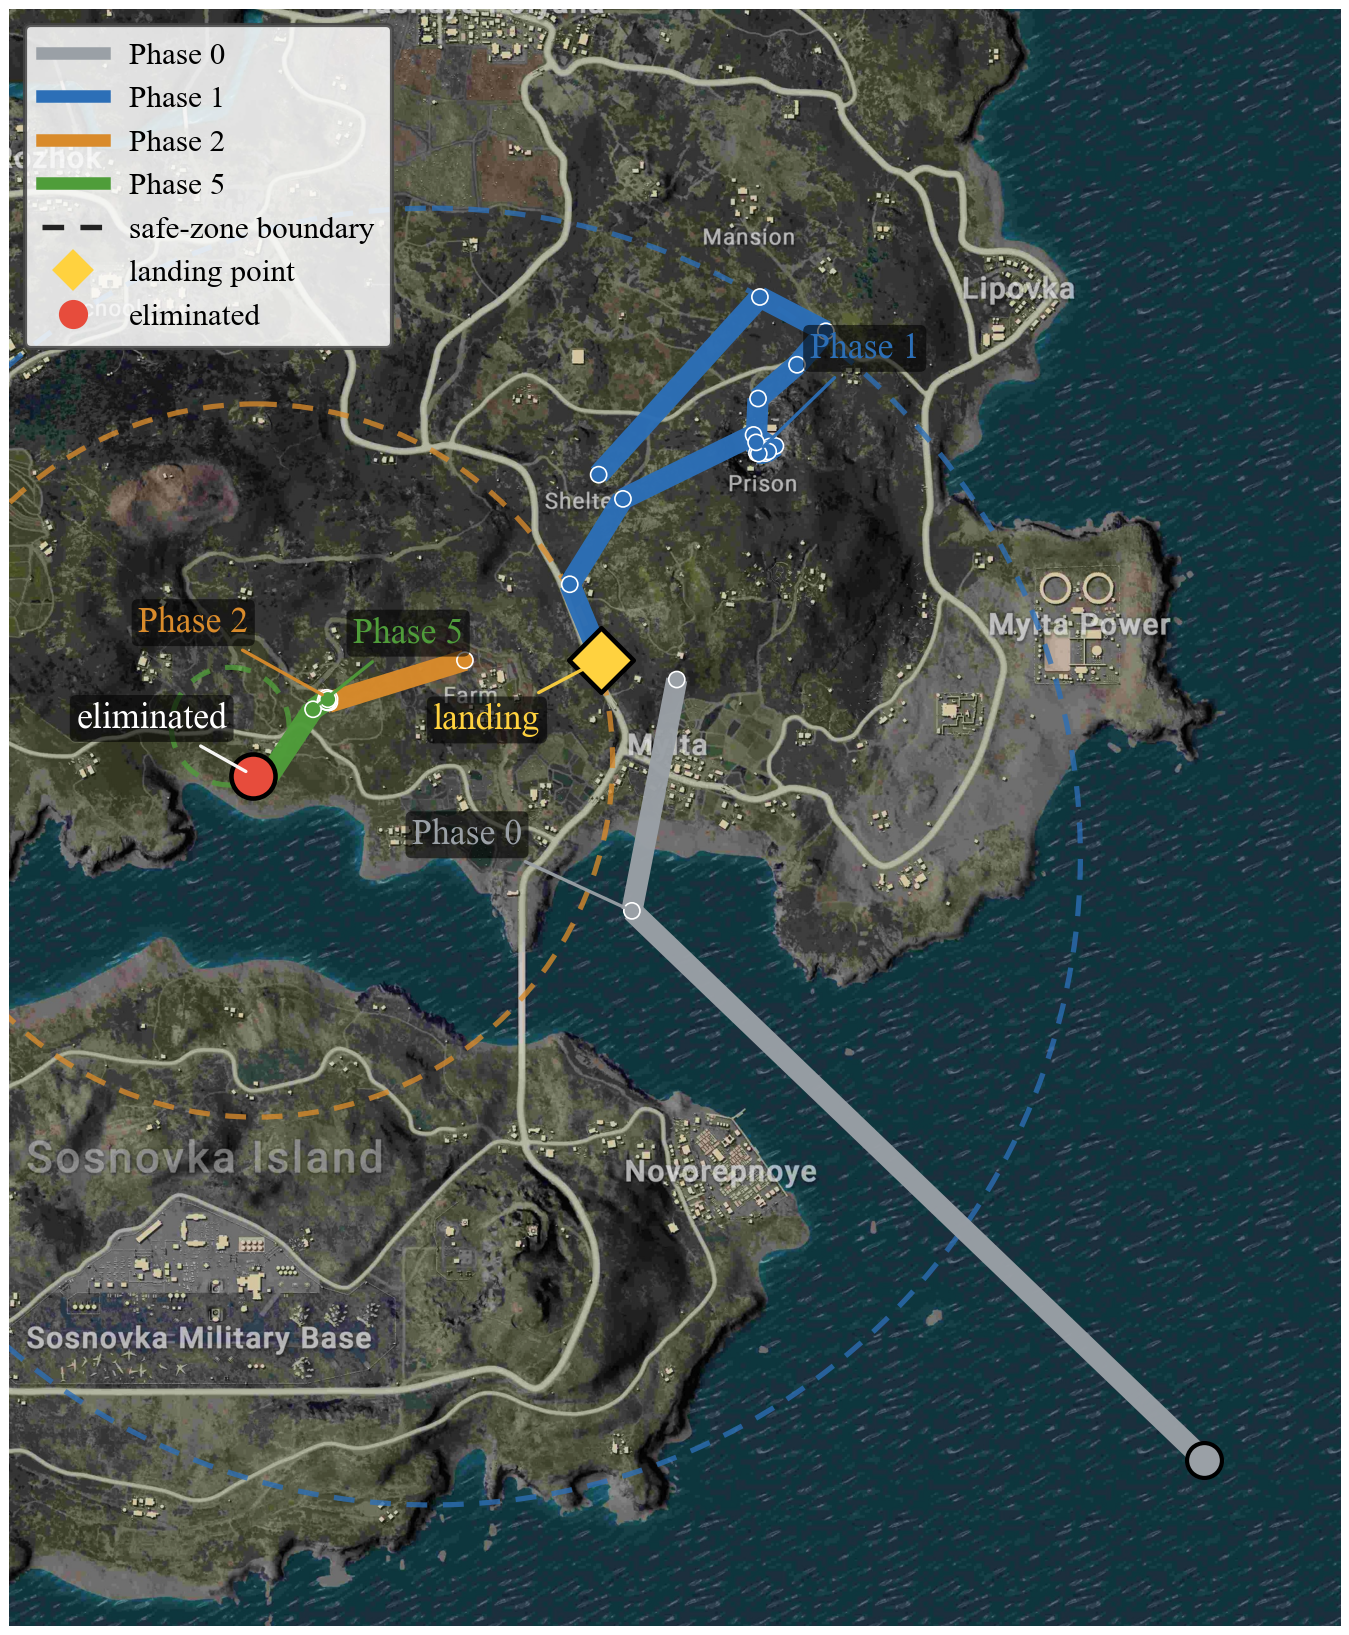
\includegraphics[width=0.48\textwidth]{figures/team_phase_feature_example.png}
\caption{PUBG gameplay as a spatio-temporal process. Solid line segments show
one team's centroid movement during selected phases, and dashed circles of the
same color show the corresponding target safe-zone boundaries on the Erangel
battlefield. Phase 0 denotes the pre-zone landing interval, the yellow diamond
marks the landing point, and the red marker denotes elimination.}
\label{fig:team-phase-feature-example}
\end{figure}

Table~\ref{tab:feature-groups} separates conventional telemetry aggregates
from the added STDB spatio-temporal features. The complete dictionary of all
66 node features, with the definition and scaling of each, is given in
Appendix~\ref{app:features}. The \(d\) column reports the raw tabular variable
count used in the HGB representation ablation; DynamicSTGNN uses normalized
numeric variants of the same sources as a 66-dimensional node feature vector.
The STDB-only count includes the shared phase index, which is counted once in
the combined view. Each quantity is scaled by a fixed, feature-specific
constant. Variables that can occasionally take very large values, such as
damage, item pickups, and combat-event counts, are log-compressed; the scales
are constants of the representation, not statistics fitted on training data.

\begin{table}[t]
\centering
\caption{Conventional telemetry aggregates and added STDB spatio-temporal
features.}
\label{tab:feature-groups}
\scriptsize
\setlength{\tabcolsep}{2.5pt}
\begin{tabular}{p{0.18\linewidth}p{0.22\linewidth}rp{0.42\linewidth}}
\toprule
Source & Group & \(d\) & Representative quantities \\
\midrule
Conventional & Phase/team state, combat, readiness & 57 &
Phase index and duration, alive teams/players, zone radii and center shift,
health, team spread, vehicles, damage, knockdowns, kills, items, healing/boost
use. \\
Added STDB & Trajectory, zone/enemy exposure & 16 &
Team-centroid path length, displacement, sinuosity, speed, rotation timing,
safe-zone alignment and entry time, boundary distance, outside-zone ratio,
enemy density, nearest-enemy distance, combat-area passage. \\
Combined view & Conventional+STDB & 72 &
Tabular hazard-prediction view combining conventional aggregates with STDB
trajectory/exposure features. \\
\bottomrule
\end{tabular}
\end{table}

\subsection{Dynamic Team Graphs (RQ1)}
\label{sec:team-graphs}

The third representation object makes inter-team relations explicit. For
phase \(k\) we define a weighted heterogeneous graph
\(G_k=(V_k,X_k,\{A_k^r\}_{r\in R})\), where \(V_k\) is the set of co-observed
teams, \(X_k\) is the team-phase feature matrix of
Subsection~\ref{sec:methods-features}, and \(A_k^r\) is the weighted
adjacency matrix of relation \(r\)~\cite{sanchezLengeling2021gnnIntro}. A
match is therefore a discrete-time dynamic graph: a sequence
\(G_1,\dots,G_T\) of snapshots, one per phase, in which nodes drop out as
teams are eliminated. All edges are computed from phase-\(k\) observations
only.

The relation set \(R\) has three channels:
\[
A^{\mathrm{prox}}_{ij,k}=e^{-\bar d_{ij,k}/\lambda},\qquad
A^{\mathrm{comb}}_{ij,k}=\log\!\big(1+D_{ij,k}+\gamma_e E_{ij,k}+\gamma_k K_{ij,k}\big),
\]
\[
A^{\mathrm{press}}_{ij,k}=\rho_{ij,k}\, e^{-\bar d^{\,\mathrm{p}}_{ij,k}/\lambda},
\]
where \(\bar d_{ij,k}\) is the mean centroid distance between teams \(i\) and
\(j\) during the phase; \(D\), \(E\), and \(K\) are the damage, eliminations,
and knockdowns dealt by \(i\) to \(j\); a team is under zone pressure when it
is outside the safe zone or within \(\tau_b\) of its boundary;
\(\rho_{ij,k}\) is the fraction of the phase that both teams jointly spend
under pressure within \(\tau_d\) of each other; and \(\bar d^{\,\mathrm p}\)
averages distance over those moments. Proximity is symmetric and complete (no
hard distance cutoff), co-pressure is symmetric and sparse, and combat is
directed and sparse. The constants are fixed a priori at map scale,
\(\lambda=200\)\,m, \(\gamma_e=100\), \(\gamma_k=50\), \(\tau_b=150\)\,m,
\(\tau_d=200\)\,m; we did not tune them, and sensitivity to these choices is
discussed in the limitations. Averaged over phases 1--8, a phase graph
contains about 14 co-observed teams, with about 14 directed combat edges and
7 co-pressure pairs per phase.

Each channel is row-normalized,
\(\bar A^{r}_{ij,k}=A^{r}_{ij,k}/\sum_{j'}A^{r}_{ij',k}\), with edgeless rows
staying zero; the proximity channel carries self-loops, and padded or
eliminated teams carry no edges at all. Two conventions matter for reading
the model. First, combat is stored with the attacker as the row: in the
aggregation \(\bar A H\), an attacking team aggregates the state of the teams
it damaged, while the converse signal---being attacked---is carried by the
combat-taken node features. Second, row normalization removes scale
differences in aggregation; absolute combat intensity is retained in
node-level combat features, so the combat adjacency encodes the distribution
of engagement partners rather than raw magnitude.
Figure~\ref{fig:dynamic-graph-example} illustrates the conversion.

\begin{figure*}[t]
\centering
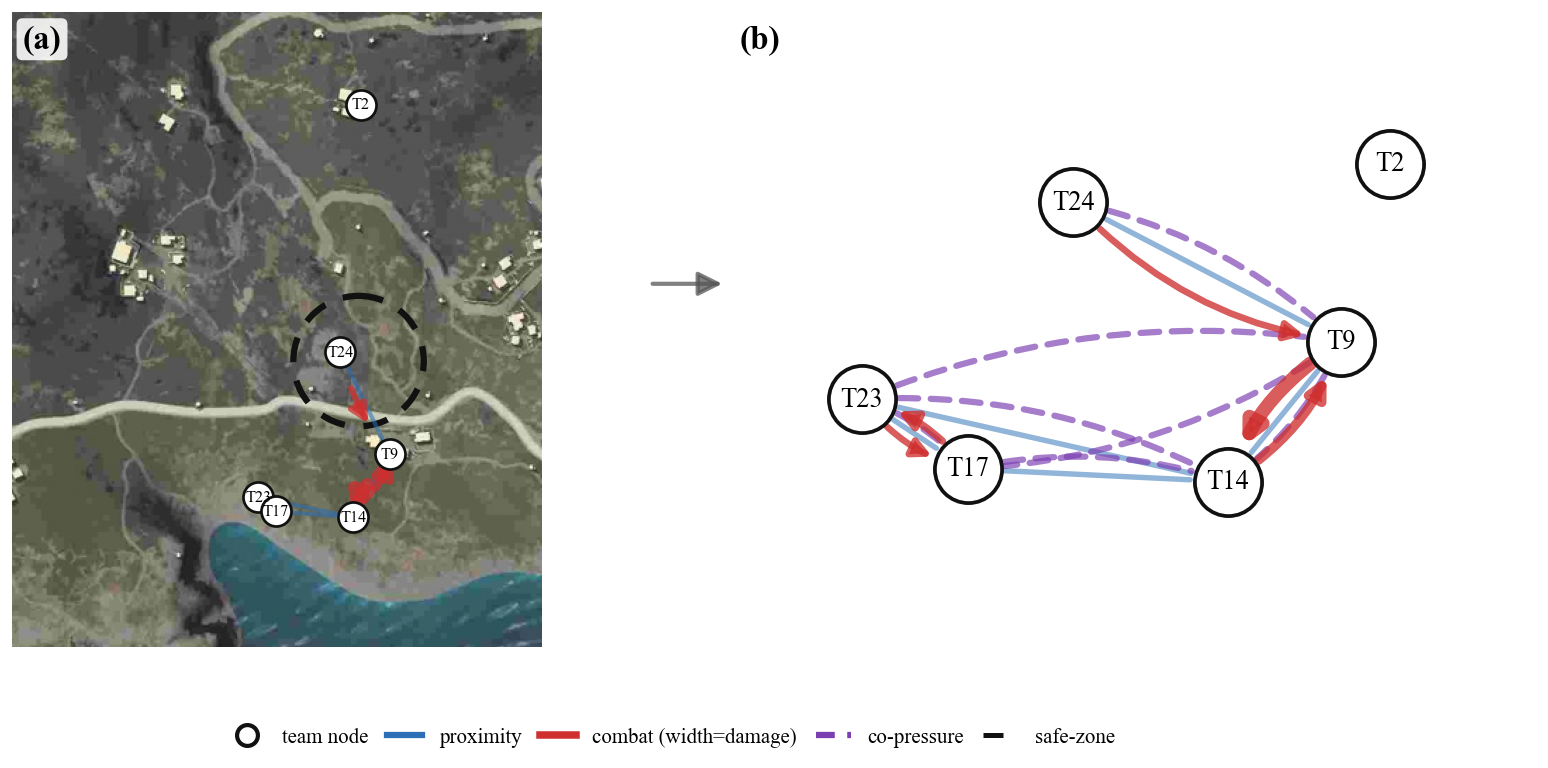
\includegraphics[width=0.86\textwidth]{figures/dynamic_heterogeneous_graph_example.png}
\caption{Visual conversion of a phase-level STDB snapshot into a dynamic team
graph for one PUBG phase. Panel (a) shows team centroids on the Erangel map,
the current safe-zone boundary, and combat events. Panel (b) keeps the same
teams and relations but removes the map background, leaving only the graph
structure used by the model.}
\label{fig:dynamic-graph-example}
\end{figure*}

This design has four properties we rely on. Heterogeneous channels keep
distinct risk mechanisms separate---being near a team, being shot by it, and
being pushed into the same shrinking space are different relations---and let
the model weigh them rather than conflating them in a single graph. The
complete weighted proximity channel avoids a distance-threshold
hyperparameter and preserves the full ordering of distances; it risks
over-smoothing in team-dense early phases, but the exponential decay
concentrates mass on nearby teams, and the no-edge and shuffle controls of
Subsection~\ref{sec:dynamic-team-graph-model} bound how much of any gain
could come from indiscriminate mixing. Directed combat edges retain who
initiated an interaction. Finally, snapshot dynamics align the graph clock
with the phase clock of the hazard task, and row normalization keeps neighbor
aggregation comparable as the number of surviving teams shrinks across
phases.

\subsection{Next-Phase Hazard Prediction Task (RQ2-i)}
\label{sec:prediction-task}

Part (i) of RQ2 asks how accurately next-phase team elimination can be
predicted from the features of Subsection~\ref{sec:methods-features} alone.
We call \(k\) the \textit{cut phase}: the model observes a match through the
end of phase \(k\) and predicts whether team \(i\) is eliminated during phase
\(k{+}1\). All inputs---features, edges, and masks---are constructed from
telemetry observable up to \(b_k\); events and outcomes after \(b_k\) enter
only the label definition.

Let \(b_k\) be the end time of phase \(k\), and \(T_i\) the elimination time
of team \(i\)---the moment its last surviving member is eliminated. The label
and hazard are
\[
Y_{i,k}=\Ind\!\left\{b_k < T_i \leq b_{k+1}\right\}, \qquad
h_{i,k}=P(b_k < T_i \leq b_{k+1}\mid T_i>b_k, X_{i,\leq k}).
\]
Teams eliminated before \(b_k\) leave the risk set and are masked. Surviving
teams contribute \(Y_{i,k}=0\) for every observed interval; once the match
ends or the eight-phase horizon is reached, their later intervals are
unobserved and treated as right-censored rather than labeled. Modeling uses
phases 1--8 and excludes the landing interval, so cut phases run from 1 to 7.
Training minimizes the masked discrete-time survival likelihood
\[
\mathcal{L}_{\mathrm{haz}}
= -\sum_{(m,i,k)\in \mathcal{R}}
\Big[ Y_{i,k}\log \hat h_{i,k} + (1-Y_{i,k})\log\big(1-\hat h_{i,k}\big) \Big],
\]
where the risk set \(\mathcal{R}\) contains exactly the team-phase cells with
\(T_i>b_k\) and an observed next phase; censored cells are excluded by the
mask. Splits are made by match, never by row. We answer part (i) in two ways:
by the absolute performance of feature-only models, and by a representation
ablation that degrades the feature set toward prior-style strategy scores
(Section~\ref{sec:experiments}).

\subsection{DynamicSTGNN (RQ2-ii)}
\label{sec:dynamic-team-graph-model}

Part (ii) of RQ2 asks whether the dynamic team graphs of
Subsection~\ref{sec:team-graphs} add predictive signal beyond the team-phase
features. DynamicSTGNN receives
\(X \in \mathbb{R}^{B \times T \times N \times F}\) and
\(A \in \mathbb{R}^{B \times T \times E \times N \times N}\), with \(T{=}8\)
phases, \(N_{\max}{=}128\) teams, \(F{=}66\) node features, and \(E{=}3\)
relation channels; Figure~\ref{fig:dynstgnn-arch} shows the architecture.
\(N_{\max}\) is a padding bound covering the largest team count across modes
(up to 100 in solo); padded nodes carry no edges and are masked throughout.
An input layer embeds each node into a 64-dimensional state \(H\), and two
identical spatio-temporal blocks follow. Each block applies a gated causal
temporal convolution, the heterogeneous graph convolution
\[
H' = \mathrm{ReLU}\Big(\sum_{r\in R} \alpha_r\, \bar{A}_k^r H W_r + H W_0\Big),
\qquad \alpha = \mathrm{softmax}(a),
\]
where \(\bar{A}_k^r\) is the row-normalized adjacency of relation \(r\),
\(W_r\) and \(W_0\) are learned projections, and \(a\) are learned channel
logits, and then a second gated causal temporal convolution with layer
normalization and a residual connection. The channel weights \(\alpha\) are
global scalars rather than phase- or team-conditioned attention; the graph
module is therefore designed to test whether the relation channels contain
additional signal, not to model context-dependent relation importance.

Although the tensor has \(T{=}8\) slots, the model emits one hazard logit per
cut phase \(k=1,\dots,7\). Temporal convolutions are left-causal, layer
normalization is applied over the feature dimension of each team-phase state
(never across time), and padded phases and eliminated teams are masked in
message passing and in the loss. A small head maps each team-phase state to
the next-phase hazard logit of Subsection~\ref{sec:prediction-task}. The full
model has about 0.34M parameters.

\begin{figure*}[t]
\centering
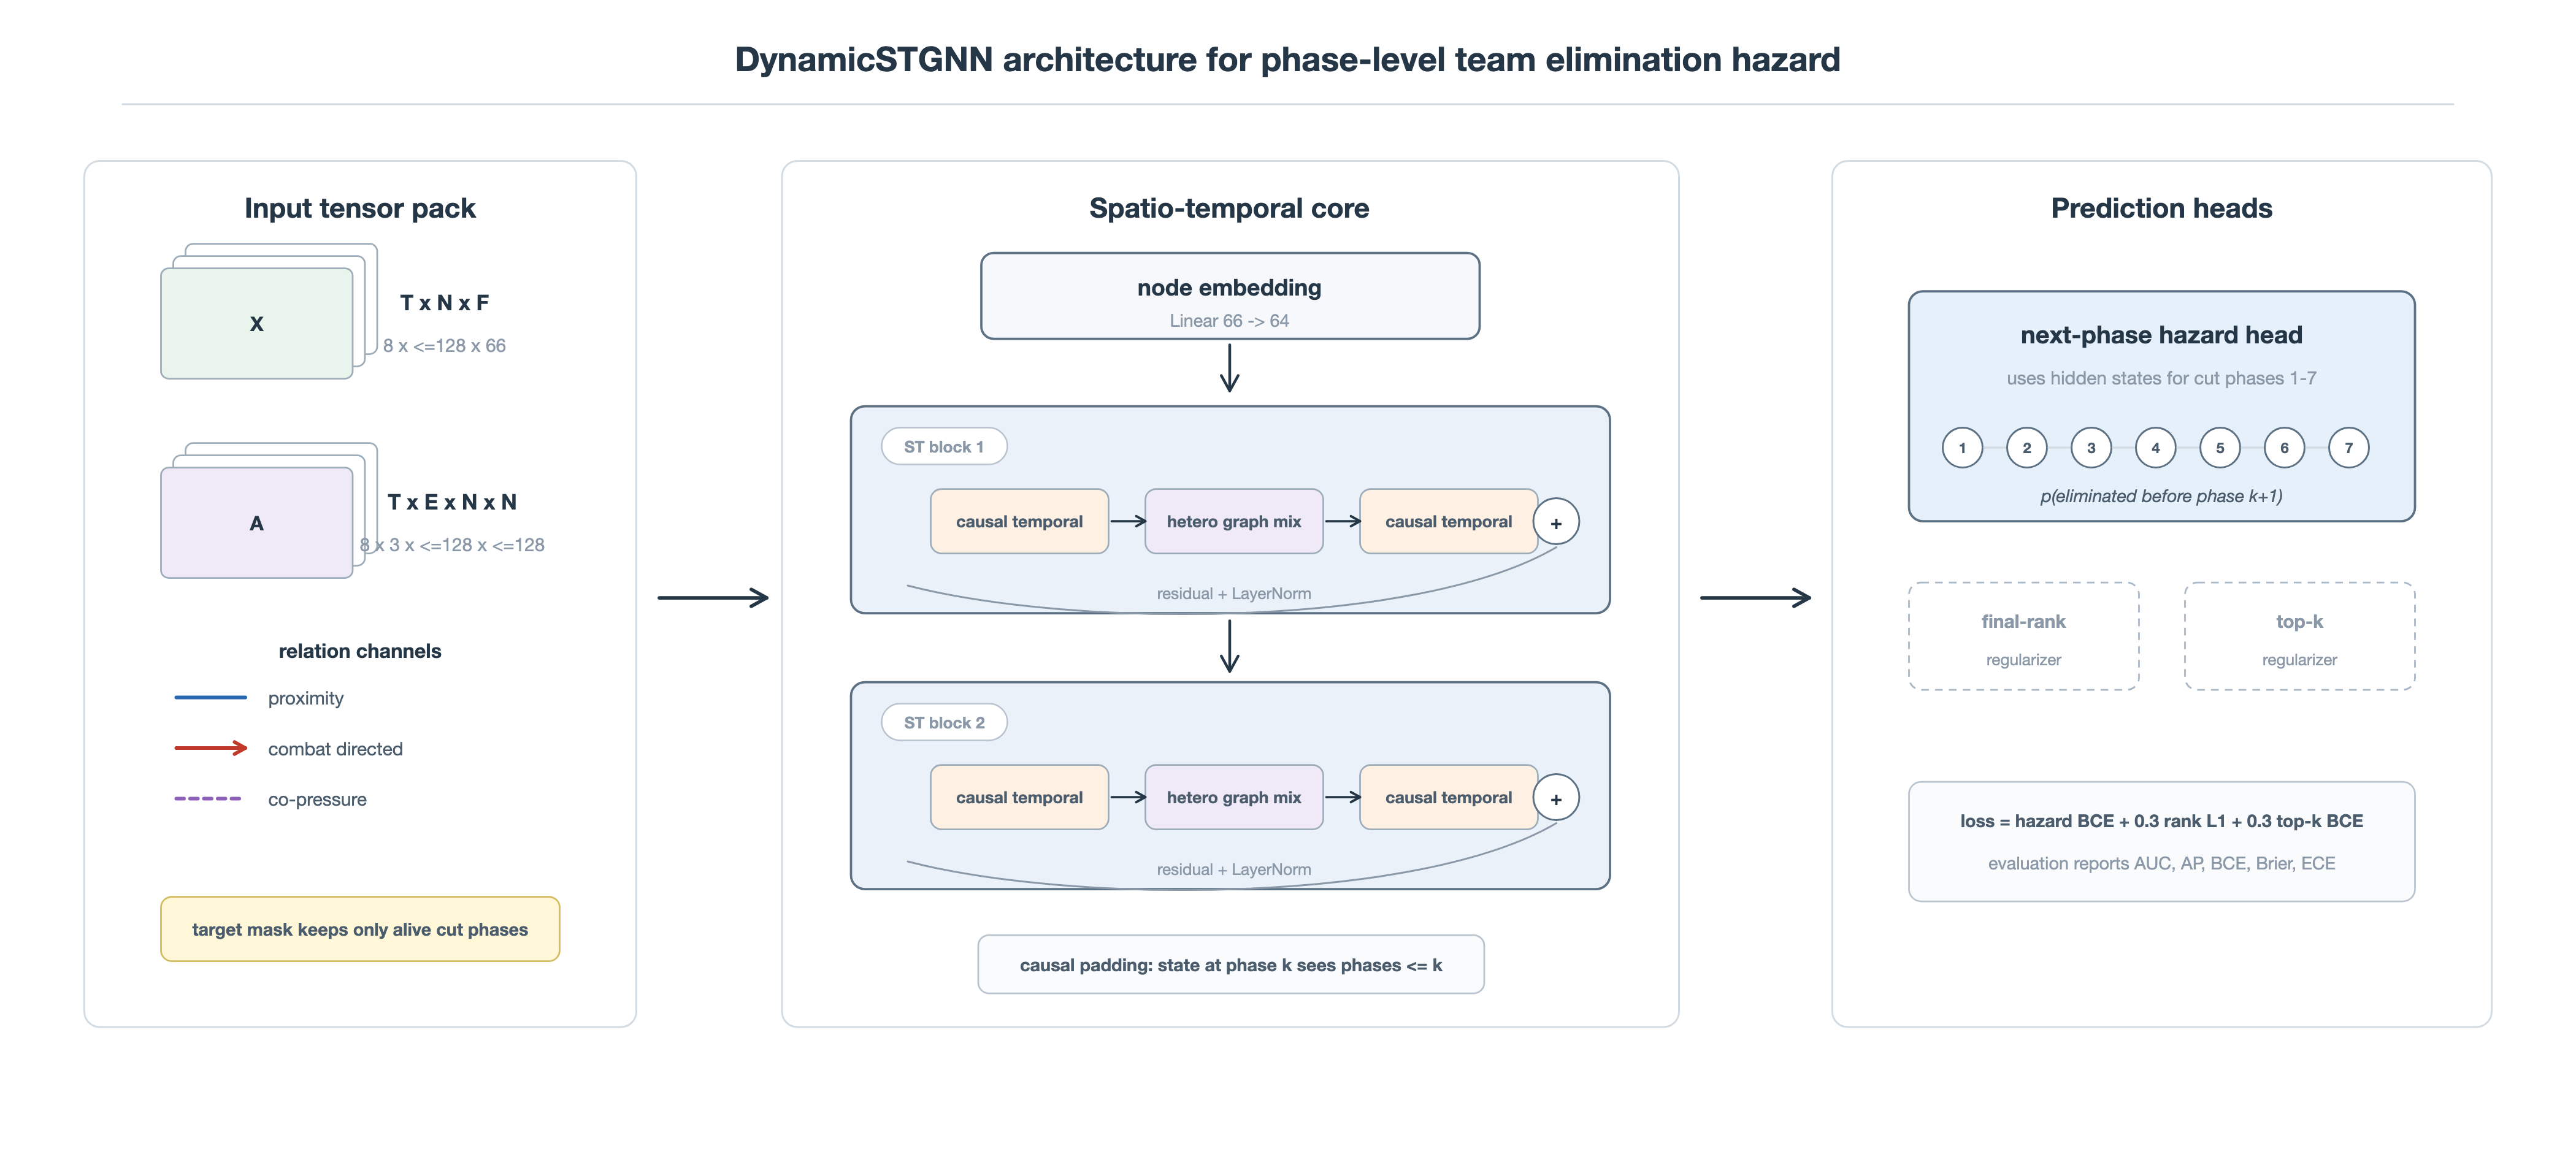
\includegraphics[width=0.86\textwidth]{figures/dynstgnn_architecture.png}
\caption{DynamicSTGNN. (a) The input is one heterogeneous team graph per
phase, with proximity, combat, and co-pressure relation channels. (b) The
network embeds node features and stacks two gated spatio-temporal blocks
before the hazard head. (c) Each ST block applies a gated causal temporal convolution, a heterogeneous graph
convolution that aggregates per relation channel and mixes channels with
learned softmax weights plus a skip connection, a second gated temporal
convolution, and layer normalization with a residual connection. Causal
padding keeps phase \(k\) from seeing later phases.}
\label{fig:dynstgnn-arch}
\end{figure*}

We compare four edge conditions: no edges, proximity only, proximity plus
combat, and the full graph. We also compare against a histogram gradient
boosting baseline on a tabular view of the same team-phase rows. The two
references play distinct roles: the boosting baseline tests whether the graph
model beats a strong tabular learner on the same representation, while the
no-edge DynamicSTGNN controls for architecture, temporal convolution, and
parameter count with relational adjacency removed. Both references already receive hand-crafted neighbor summaries
(nearby enemy density, nearest-enemy distance) among the node features, so
improving on them attributes the gain to relational structure beyond what
such summaries capture. Only gains over both references support the claim
that dynamic team relations add predictive signal. Two controls guard this
conclusion further: shuffling team identities within the observed graphs at
inference time should erase the gain if it truly comes from who relates to
whom, and the gain should persist when training is repeated under different
random seeds.

